% !TeX spellcheck = en_US
% !TeX encoding = UTF-8
\section{Metadynamics\label{Sec:ES:metadynamics}}
Metadynamics was first suggested by Laio and Parrinello in 2002.\cite{LaioPNAS2002} Imaging you became Doraemon in a dream. You were standing in a valley and were surrounded by high mountains. In most of the time, you are just wandering near the minimum, because your kinetic energy is not enough to climb the mountains. Suddenly, you realize that you can use metadynamics as a magic to escape from the minimum. After each step, you took a bottle of sand out of your miraculous pocket and put the sand under your feet. Then you were lifted inch-by-inch, and the chance of visiting where you had visited became less and less. And you were finally raised up to the top of the mountain and at that moment you was able to climb over that mountain without much effort and fell into another valley. The magic of sand continued, and at last you smoothed the whole area. Because you wrote diaries every day and you have all the records on where you had put the sand and how much sand you had put there. You drew the shape the piled sand according to the record and you flipped it. At that moment, you got the exact shape of the original free energy landscape. 
\begin{figure}[htbp]
	\centering
	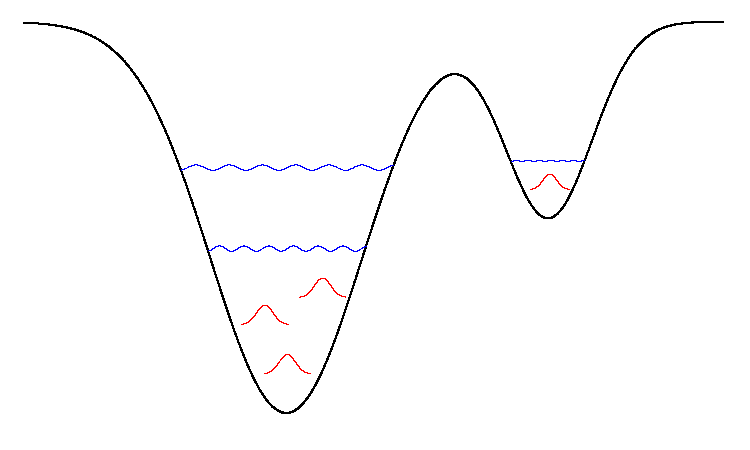
\includegraphics[width=0.6\textwidth]{figures/metadynamics.pdf}\\
	\caption{}\label{Fig:ES:metadynamics}
\end{figure}